\chapter*{B}

\section*{Bugle calls}

The Cheshire Yeomanry typically used the calls of the 5\nth Royal Inniskilling Dragoon Guards~\cite[p11]{trumpet-and-bugle-calls}, but also had their own trumpet and bugle calls.

\begin{figure}[h]
  \centering
  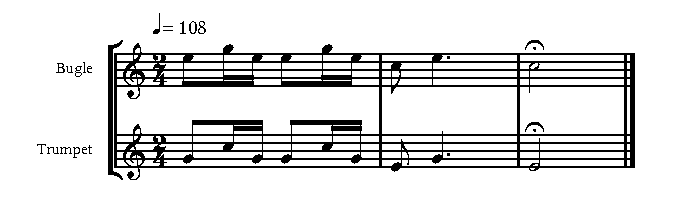
\includegraphics[width=0.75\textwidth]{gazette/cheshire-yeomanry-call.pdf}
  \caption*{Regimental call of the Cheshire Yeomanry~\cite[p11]{trumpet-and-bugle-calls}}
\end{figure}

\begin{figure}[h]
  \centering
  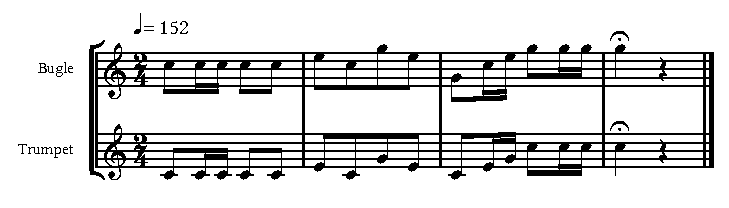
\includegraphics[width=0.75\textwidth]{gazette/5ridg-call.pdf}
  \caption*{Regimental call of the 5\nth Royal Inniskilling Dragoon Guards~\cite[p3]{trumpet-and-bugle-calls}}
\end{figure}
